% ------------------------------------------------------------------------
% ------------------------------------------------------------------------
% abnTeX2: Modelo de Trabalho Acadêmico em conformidade com 
% as normas da ABNT
% ------------------------------------------------------------------------
% ------------------------------------------------------------------------

\documentclass[english, 
               brazil, 
               bsc] %Opções bsc (TCC) e msc (Mestrado)
               {dcomp-abntex2}

% Geração de dummy text
% Retirar para a versão final do documento
\usepackage{lipsum}
\usepackage{multirow}
\usepackage{trivfloat}
\trivfloat{quadro}

%Compila o indice
\makeindex

\begin{document}

% Seleciona o idioma do documento (conforme pacotes do babel)
\selectlanguage{brazil}

% Retira espaço extra obsoleto entre as frases.
\frenchspacing 

% ----------------------------------------------------------
% ELEMENTOS PRÉ-TEXTUAIS
% ----------------------------------------------------------
\pretextual

\titulo{Gerenciamento de controladores SDN com aplicações para propósitos de segurança}
\autor{Carolina Santana Louzada}
\orientador{Ricardo José Paiva de Britto Salgueiro}
\coorientador{Edilayne Meneses Salgueiro}
\curso{Engenharia de Computação}

\imprimircapa
\imprimirfolhaderosto*

   
\begin{dedicatoria}
   \vspace*{\fill}
   \centering
   \noindent
   \textit{ Dedico este trabalho primeiramente a Deus, que é meu guia; à toda minha família, principalmente, minha mãe, que me deu todo apoio, compreendendo minhas ausências ao longo dos períodos; ao meu namorado, Gabriel, que também esteve sempre ao meu lado me motivando durante minhas dificuldades e me compreendendo; aos meus amigos de curso, que também estiveram presentes nos desafios do curso, fracassos e sucessos; e aos professores que me deram orientação e todo o suporte para que eu chegasse aqui.} \vspace*{\fill}
\end{dedicatoria}
% ---
\begin{agradecimentos}

%lipsum[1-4] 
 Agradeço ao Prof. Ricardo José Paiva de Britto Salgueiro e à Prof. Edilayne Meneses Salgueiro por me orientarem na produção deste trabalho e por me motivarem a continuar trilhando o caminho da educação e da pesquisa. Agradeço também à Marco Aurélio Cruz Fonseca, que percorreu comigo os desafios deste trabalho, me ensinando e também aprendendo junto a mim.
\end{agradecimentos}
% ---
\begin{epigrafe}[]
    \vspace*{\fill}
	\begin{flushright}
	
		\textit{
				“A verdadeira viagem de descobrimento \\ não consiste em procurar novas paisagens,\\ mas em ter novos olhos”. (Marcel Proust)
				}
		
	\end{flushright}
\end{epigrafe}
% ---
%% resumo em português
\setlength{\absparsep}{18pt} % ajusta o espaçamento dos parágrafos do resumo
\begin{resumo}
  


 \textbf{Palavras-chave}: 
\end{resumo}
%% resumo em inglês
\setlength{\absparsep}{18pt} % ajusta o espaçamento dos parágrafos do resumo
\begin{resumo}[Abstract]
 \begin{otherlanguage*}{english}
   

   \textbf{Keywords}: Algorithms, DataBase, Cloud Computing, Lero-Lero.
 \end{otherlanguage*}
\end{resumo}
    
% Lista de Figuras
\pdfbookmark[0]{\listfigurename}{lof}
\listoffigures*
\cleardoublepage

% Lista de Tabelas
\pdfbookmark[0]{\listtablename}{lot}
\listoftables*
\cleardoublepage

% Lista de Códigos
%\pdfbookmark[0]{\listlistingname}{lol}
%\begin{KeepFromToc}
%	\listoflistings
%\end{KeepFromToc}
\cleardoublepage
   
% ---
% inserir lista de abreviaturas e siglas
% ---

\begin{siglas}
    \item[SDN]{Software-Defined Networking}
	\item[API]{Application Programming Interface}
	\item[DoS]{Denial of Servie}
	\item[IP]{Internet Protocol}
	\item[MAC]{Media Acess Control}
	\item[RFC]{Requests for Comments}
	\item[PC]{Personal Computer}
	\item[WAN]{Wide Area Network}
	\item[NIB]{Network Information Base}
	\item[AMQP]{Advanced Message Queuing Protocol}
	\item[RSVP]{Resource Reservation Protocol}
	\item[REST]{Representational State Transfer}
	\item[WEB]{World Wide Web}
	\item[VM]{Virtual Machine}

\end{siglas}
% ---
%% ---
% inserir lista de símbolos
% ---

\begin{simbolos}
  \item[$ \Gamma $] Letra grega Gama
  \item[$ \Lambda $] Lambda
  \item[$ \zeta $] Letra grega minúscula zeta
  \item[$ \in $] Pertence
\end{simbolos}
% ---
    
\pdfbookmark[0]{\contentsname}{toc}
\tableofcontents*
\cleardoublepage

% ----------------------------------------------------------
% ELEMENTOS TEXTUAIS
% ----------------------------------------------------------
\textual
\chapter{Introdução}

\section{Contextualização}

O desenvolvimento das redes tradicionais de computadores, principalmente, quando se fala em redes corporativas, envolve o aumento da infraestrutura física, o que implica também no aumento da complexidade de gerenciamento de elementos físicos como roteadores e \emph{switches}. Os equipamentos mais modernos normalmente são formados pela camada ou plano de controle e de dados, os quais possuem funções diferentes. A camada de controle é responsável pela lógica de encaminhamento dos dados no nível físico, logo, ele dita como o \emph{switch} deve lidar com os dados que passarem por ele. O plano de dados já é responsável por lidar com os dados propriamente ditos, os encaminhando para outros \emph{switches} e cumprindo com o que lhe foi atribuído pelo plano de controle. O maior desafio para as redes convencionais se encontra no fato que os elementos físicos possuem seus planos de controle configurados pelo próprio fabricante. Nesse contexto, quando se fala em redes heterogêneas, o gerenciamento se torna muito mais complexo para os administradores, que precisam lidar com diferentes tecnologias e diferentes protocolos. Esse desafio limita o desenvolvimento de experimentos e novas tecnologias para redes, tornando necessário que se estude novas abordagens que solucionem essa limitação.
\par As Redes Definidas por Software surgiram neste cenário como solução para esses problemas decorrentes nas redes convencionais. As ideias por trás das redes programáveis surgiram a partir do final dos anos 90 com as redes ativas. Já por volta do início dos anos 2000 surgiu o conceito da separação dos plano de controle e de dados, uma das principais características das redes SDN. A partir de 2007, o projeto Ethane deu início à utilização de interfaces abertas nas redes SDN, possibilitando que o OpenFlow fosse implementado e posteriormente fosse viabilizado como interface \emph{SouthBound} padrão das redes SDN.\cite{Feamster:2013:RS:2559899.2560327} Dessa forma, as Redes Definidas por Software chegaram à arquitetura atual, onde o plano de controle é responsabilidade dos controladores SDN e o plano de dados permaneceu em função dos elementos físicos de encaminhamento, como roteadores e \emph{switches}.
\par Por ser tão recente, as redes SDN ainda enfrentam muitos desafios, principalmente em torno da segurança de dados. Isso se deve porque as soluções atualmente existentes levam em consideração ataques nas redes tradicionais e a segurança não é uma característica inerente à arquitetura SDN. Além da modificação das ameaças das redes tradicionais, novas ameaças surgiram devido às próprias características do SDN, como centralização lógica e programabilidade da rede. Atualmente, já existem soluções que se concentram em fornecer segurança a partir de novas políticas administrativas, aplicações ligadas aos controladores e até modificações na própria arquitetura SDN.
\par Além dos desafios em torno da segurança, um outro ponto constantemente debatido é em relação à disposição dos controladores em uma rede.Sabe-se que utilizar somente um controlador, pode gerar problemas relacionados à sobrecarga do mesmo, principalmente em redes complexas. A partir de então, sugeriu-se a utilização de mais controladores, que compartilham a visão global da rede podendo se dispor de forma hierárquica ou não. Entretanto, a forma como isso deve ocorrer e como esses controladores devem se comunicar ainda é motivo de estudos e experimentos.
\par Neste contexto, este trabalho tem como propósito desenvolver um gerenciador para 2 controladores SDN em uma rede distribuída, utilizando os serviços de segurança implementados por \citeonline{pablo} e \citeonline{bomfim2}.  

\section{Objetivos}

\subsection{Objetivo Geral}

Desenvolver um gerenciador SDN para dois controladores com diferentes implementações e utilizando serviços com propósitos de segurança.

\subsection{Objetivos Específicos}

\begin{itemize}
    \item Analisar arquitetura dos controladores a serem gerenciados;
    \item Projetar módulo de gerenciamento para 2 controladores pré-definidos, elicitando seus requisitos, de forma que seja escalável para outros controladores;
    \item Analisar performance desse controlador;
\end{itemize}


\section{Estrutura do Documento}

Para facilitar a navegação e melhor entendimento, este documento está estruturado com os seguintes capítulos:
\begin{itemize}
\item {Capítulo 1 - Introdução} 
\item {Capítulo 2 - Fundamentação Teórica}
\item {Capítulo 3 - Trabalhos Relacionados}
\item {Capítulo 4 - Metodologia}
\end{itemize}

\chapter{Fundamentação Teórica}

\section{Redes Definidas por Software}

De acordo com a \citeonline{SDNFoundation} e \citeonline{ALSMADI}, o paradigma SDN é uma arquitetura emergente que se diferencia por ser  dinâmica, gerenciável, de bom custo-benefício e com boa adaptabilidade, o que a torna ideal para aplicações que exigem alta largura de banda e ainda pela natureza dinâmica dessas aplicações.
\par A arquitetura SDN possui como principais características:

\begin{itemize}
    \item \textbf{Diretamente programável}: O controle da rede é diretamente programável devido a seu desacoplamento das funções de encaminhamento;
    \item \textbf{Ágil}: A abstração do controle de encaminhamento de pacotes por meio dos controladores permite que os administradores ajustem dinamicamente o fluxo de tráfego;
    \item \textbf{Gerenciamento Centralizado}: A inteligência lógica da rede é centralizada nos controladores, que possuem uma visão global da rede;
    \item \textbf{Programaticamente Configurável}: SDN permite que os administradores configurem, gerenciem, e otimizem sua segurança rapidamente via aplicações automatizadas para SDN, independente de softwares proprietários;
    \item \textbf{ Baseada em padrões abertos}: A implementação SDN em padrões abertos simplifica o projeto e a operação de redes.
    \item \textbf{Gerenciamento baseado em fluxos:}  Apesar do controle por fluxo também existir nas redes convencionais, os protocolos de roteamento se baseiam nos endereços IP para a tomada de decisões. Para o SDN, as decisões de encaminhamento tomam como base os fluxos que entram e saem dos \emph{switches}.
    
\end{itemize}

\subsection{Histórico}
O surgimento das Redes Definidas por Software remonta anos de pesquisas em diversas tecnologias de redes e seus paradigmas. Cada pesquisa, desejando compreender ou solucionar algum problema específico na área de redes terminou por contribuir para o desenvolvimento do que hoje chamamos de redes SDN (\textit{Software-Defined Networking}).

\begin{figure}[!h]
	\caption{ Desenvolvimento de redes programáveis com o passar dos
	anos.
}
  \centering
  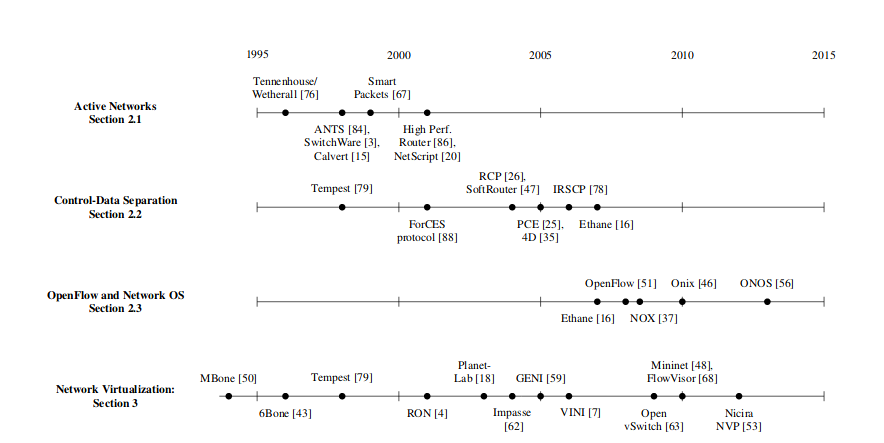
\includegraphics[scale=0.5]{Imagens/SDNHistory(1).png} 
  
  \legend{Fonte:\citeonline{Feamster:2013:RS:2559899.2560327} }
  \label{SDNHistory(1).png}
\end{figure}

\par A história do paradigma SDN, observando a Figura \ref{SDNHistory(1).png}, se inicia com o estudo de redes ativas e virtualização de redes durante os anos 90, período no qual a internet se tornou escalável e crescia rapidamente\cite{Feamster:2013:RS:2559899.2560327}.
De acordo com \citeonline{Tennenhouse:1997:SAN:2288390.2288938,Bhattacharjee:1997:AAN:267213.267289}, as redes ativas podem ser definidas como redes que possuem capacidade de expor recursos dos nós e customizar a computação de dados que passam pelos \textit{switches}, funcionalidades até então inexistentes nas redes convencionais passivas. Nesse mesmo período as pesquisas de virtualização de redes também avançavam e sua importância se dá porque a virtualização abstrai o funcionamento de uma rede, desacoplando-a da infraestrutura física de forma a diminuir a complexidade sobre a mesma. 
\par Por volta dos anos 2000, o volume de tráfego de rede continuava aumentando, e os pesquisadores buscavam balancear esse aumento de tráfego com características como confiabilidade, previsibilidade e performance da rede. Entretanto, o principal obstáculo se encontrava na integração inflexível entre o plano de controle e de dados nos roteadores e \emph{switches} convencionais. Essa integração dificultava  a exploração de novos protocolos nas redes, tornando os administradores dependentes do suporte da infraestrutura física. A partir de então outros estudos foram feitos para separar essas duas camadas, gerando inovações como a abertura de interface entre os planos de controle e de dados e também através de novas arquiteturas com centralização da lógica do controle da rede. Essas inovações são vistas respectivamente através da interface ForCES(\textit{Forwarding and Control Element Separation}) e das arquiteturas RCP (\textit{Rounting Control Protocol}) e SoftRouter.
\cite{Nunes}
\par A partir de 2005, a separação do plano de controle do plano de dados já era uma realidade, contudo, ainda era necessário experimentos em larga escala para validar as vantagens e desvantagens dessa separação, dessa forma, os campus das universidades se tornaram ambientes de experimentação de novas arquiteturas e protocolos. 

Proposto por \citeonline{Casado} e desenvolvido na Universidade de Stanford, a arquitetura Ethane foi criada como solução para gestão de redes empresariais baseada em fluxos de pacotes e programada através de linguagem de linguagem de alto nível. Sua proposta era justamente separar o plano de controle do plano de dados, colocando toda a inteligência da rede em uma infraestrutura centralizada chamada controlador que se comunicaria com um switch Ethane, composto de uma tabela de fluxos e um canal seguro de comunicação.

Tendo como base o Ethane, também foi desenvolvido na Universidade de Stanford em 2008 um protocolo aberto de comunicação entre o controlador da rede e a infraestrutura física, tornando as redes SDN finalmente viáveis: o protocolo OpenFlow, que posteriormente se tornaria padrão de interface na arquitetura SDN.\cite{McKeown:2008:OEI:1355734.1355746} 

A partir de então o protocolo OpenFlow tem sido constantemente desenvolvido para prover melhores soluções para os problemas surgidos pela própria arquitetura SDN estando atualmente na versão 1.5, de acordo com \citeonline{SDNFoundation} . Dada sua importância para as redes SDN, mais detalhes de seu funcionamento serão expostos em uma subseção futura.

\subsection{Arquitetura SDN}

  A arquitetura SDN pode ser descrita de forma simplificada como na Figura \ref{SDN.png}. Os \emph{switches} e roteadores ligados aos sistemas finais se comunicam com o controlador SDN de forma que este possa ter uma visão global da rede e tome decisões dinamicamente com base no estado atual da rede, repassando estas decisões aos elementos físicos.

   \begin{figure}[!h]
	\caption{ Elementos da arquitetura SDN}
  \centering
  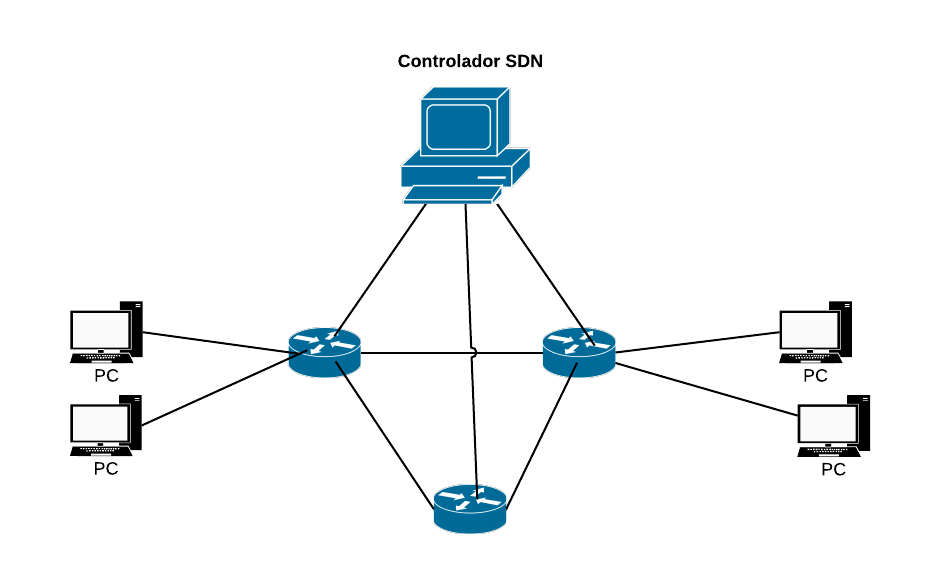
\includegraphics[scale=0.3]{Imagens/SDN.png} 
 
  \legend{Fonte: Autoria própria}
  \label{SDN.png}
\end{figure}
 
   De forma mais detalhada, de acordo com a Figura \ref{ArquiteturaSDN.png}, a arquitetura SDN  é dividida em 3 camadas: camadas de aplicação, de controle e de infraestrutura.\cite{Nunes}
   
\begin{figure}[!h]
    \caption{ Detalhamento da arquitetura SDN.}
    \centering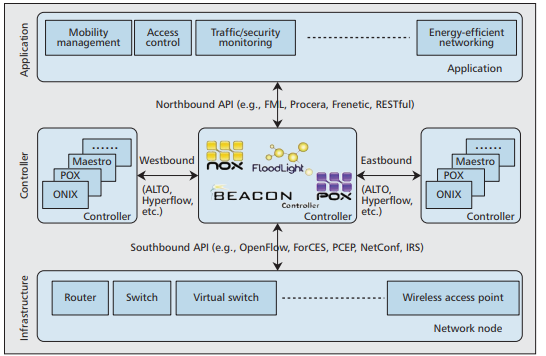
\includegraphics[scale=0.8]{Imagens/ArquiteturaSDN.png}
    \legend{Fonte: \citeonline{Sezer}}
    \label{ArquiteturaSDN.png}
\end{figure}
   
   \subsubsection{Camada de Infraestrutura}
   
   Também chamada de plano de dados ou de encaminhamento. Nesta camada concentram-se elementos de encaminhamento de pacotes, como switches(virtuais ou físicos) e roteadores, que devem ser programáveis e capazes de se comunicar com o controlador através das chamadas \emph{APIs SouthBound}. No paradigma SDN, apesar da existência de diversas \emph{APIs SouthBound}, o uso do Protocolo Openflow já é bastante difundido e tido como padrão para comunicação entre o plano de dados e de controle.\cite{kreutz} 

\subsubsection{Camada de Controle}

 Na camada de lógica e controle de dados, encontram-se os controladores, que são responsáveis por monitorar e modificar o comportamento dos dispositivos do plano de dados, tendo uma visão global da rede. Estes podem ser implementados em diversas linguagens e ainda serem conectados a outros controladores na mesma rede através das \emph{APIs Eastbound}, já as \emph{APIs Westbound} são responsáveis por prover comunicação entre dispositivos legados de rede. De modo a facilitar o gerenciamento e programação da rede, os controladores são vistos como sistemas operacionais de rede, pois utilizam uma interface de programação de alto nível para os operadores, abstraindo  a complexidade da camada de infraestrutura.\cite{McKeown:2008:OEI:1355734.1355746}
       
\subsubsection{Camada de Aplicação}

No nível mais alto da arquitetura temos a camada de aplicação ou gerenciamento, que se conecta com os controladores através das \emph{APIs Northbounds}. Essas interfaces são também importantes na arquitetura SDN, pois ao considerarmos os controladores como os sistemas operacionais da rede, podemos fazer uma analogia de que o mesmo necessita de outras aplicações que definam novas funcionalidades e serviços dentro do mesmo ambiente de acordo com a necessidade. Dessa forma, as aplicações de rede se tornam responsáveis de fato pelo controle lógico, cujos comandos serão traduzidos pelos controladores e enviados às entidades do plano de dados, ditando o comportamento dos mesmos.\cite{Nunes}
       
       Diferentemente da interface \emph{Southbound}, que utiliza de forma padrão o OpenFlow, essa interface ainda não possui uma proposta padronizada e comunicação entre os controladores e as aplicações que utilizarão seus serviços. De acordo com  \citeonline{kreutz}, ainda é cedo para essa padronização, pois os estudos de casos com as diferentes interfaces ainda estão ocorrendo. Contudo, é esperado que uma padronização venha a ocorrer com o desenvolvimento gradual do SDN. Além disso, as interfaces Northbound estão ligadas diretamente às implementações dos controladores, portanto, os diversos controladores existentes definem suas próprias interfaces para comunicação com a camada de aplicação. Mesmo que não seja o momento para definir uma interface \emph{Northbound} padronizada, existe o senso comum que para existir comunicação entre os diversos controladores é importante que essas interfaces sejam abertas e padronizadas, garantindo portabilidade e interoperabilidade. 
     

  
\par Diante da descrição das camadas e componentes de uma rede SDN, percebe-se que as vantagens desta quanto à separação do plano de dados e de controle se estende para diversos ambientes de rede, configurando soluções com aplicações para redes empresariais, \emph{data centers}, redes com infraestrutura \emph{wireless} e redes reais ou de pequeno porte.\cite{Nunes}


\subsection{O Protocolo OpenFlow}

O protocolo OpenFlow tornou-se tão importante no desenvolvimento das redes SDN que tornou-se padrão na interface de comunicação entre a camada de infraestrutura e controladores. Isso deu porque ele permite acesso direto aos dispositivos de encaminhamento de dados, como switches e roteadores. De acordo com SDNBOOK , o Openflow pode ser comparado a um conjunto de instruções de uma CPU. Ele especifica instruções básicas que podem ser utilizadas por aplicações externas para programar os dispositivos de rede, assim como o conjunto de instruções de uma CPU tornam possíveis programar sistemas computacionais abstraindo a complexidade do hardware.

\begin{figure}[!h]
    \caption{Componentes de um switch Openflow}
    \centering
    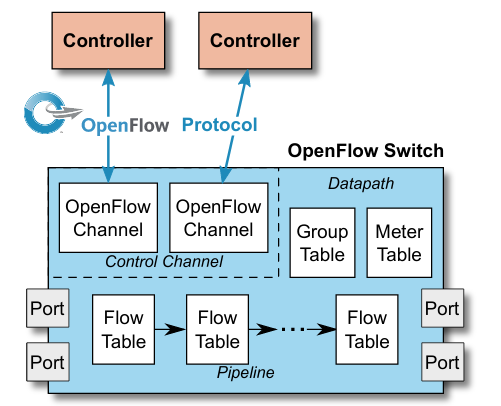
\includegraphics[scale=0.4]{Imagens/mainComponentesOpenflow.png}
    \label{mainComponents}
    \legend{Fonte: \cite{openflowSpecification}}
\end{figure}


Observando a Figura \ref{mainComponents}, percebe-se que os principais componentes Openflow são :

\begin{itemize}
    \item Controlador
    \item Switch lógico OpenFlow :
        \begin{itemize}
            \item Portas
            \item Canal Seguro
            \item Tabelas de fluxos e entradas
        \end{itemize}{}
    \item Protocolo Openflow
\end{itemize}{}


\subsection{Desafios em Redes SDN}

Os benefícios das redes SDN ainda contrastam com diversos desafios ocasionados pela própria arquitetura SDN. \citeonline{JAMMAL} em seu trabalho cita 8 desafios, ilustrados pela Figura \ref{Desafios.png}. 

\begin{figure}[!h]
    \caption{Desafios da arquitetura SDN.}
    \centering
    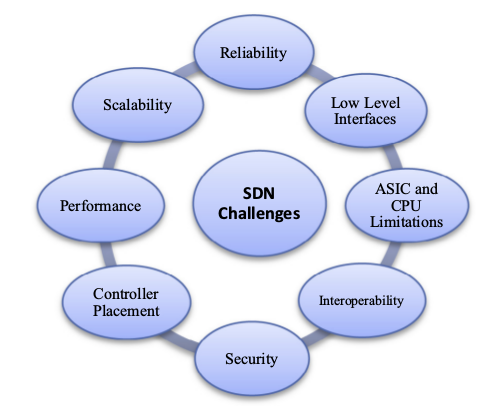
\includegraphics[scale=0.5]{Imagens/desafiosSDN.png}
    \label{Desafios.png}
    \legend{Fonte: \citeonline{JAMMAL}}
\end{figure}

\pagebreak

\begin{itemize}
    \item Confiabilidade: Em redes convencionais, quando há falha de algum dos dispositivos da rede o fluxo é desviado para outros dispositivos de forma a manter o fluxo. Entretanto, nas redes SDN a falha no controle lógico se torna um grande problema para o quesito confiabilidade, principalmente se esse controle está de fato centralizado em somente um controlador. 
    \item Escalabilidade: O desacoplamento dos planos de dados e de controle gera uma característica de interdependência na evolução das partes, contudo, também gera problemas na escalabilidade da rede. À medida que novos dispositivos físicos são inseridos e novos fluxos de rede são criados, o controlador pode passar a receber muito mais requisições do que pode processar, causando um "gargalo" na rede.
    \item Performance: A performance de uma rede SDN é medida por duas métricas: números de fluxos por segundo e tempo de configuração de fluxo. Para o caso do tempo de configuração de fluxo ainda existem os modos proativo e reativo, sendo que o último é normalmente utilizado pelo controlador SDN. Resumidamente, no modo reativo o tempo de configuração de fluxo é medido a partir do momento que o pacote chega no \emph{switch} e não há regras na tabela que especifiquem a ação sobre o mesmo. Dessa forma, o controlador toma alguma decisão sobre o pacote independente da tabela de fluxo. O tempo que o controlador leva para processar o pacote, tomar uma decisão e atualizar a tabela pode levar a problemas relacionados à latência e vazão.
    \item Posicionamento do controlador: A questão sobre a localização do controlador influencia em cada aspecto do plano de controle, seja nas latências dos fluxos até confiabilidade da rede e performance. O problema se resume em como posicionar um dado número de controladores numa certa rede física tal que suas funcionalidades sejam otimizadas para um objetivo específico.
    \item Limitações da CPU: As limitações da CPU no \emph{switch} afetam a banda entre este e o controlador. Esse quesito também afeta diretamente a questão da escalabilidade.
    \item Uso de interfaces de baixo nível entre controlador e dispositivos de rede: Apesar do SDN simplificar o gerenciamento de redes através das interfaces simplificadas para determinar políticas de rede de alto nível, o \emph{framework} das camadas inferiores precisam traduzir essas políticas para configurações de baixo nível no \emph{switch}.
    \item Segurança: A separação do plano de dados e controle tornou o gerenciamento de redes mais simplificado e dinâmico, contudo a segurança não é um quesito embutido nas características da arquitetura. Além disso, as tecnologias atuais de segurança foram pensadas especificamente para redes convencionais e justamente por ser um paradigma emergente, as redes SDN ainda não estão totalmente padronizadas, gerando ainda mais desafios para o quesito segurança.
    
\end{itemize}


\section{Conceitos de Segurança de Redes}

\par Gerenciar redes de computadores em um cenário com tantos usuários, grande volume de dados e diversidade tecnológica gerou novas vulnerabilidades nos sistemas, tornando-se um desafio para os pesquisadores da segurança de informação. Isso ocorre porque de acordo com \citeonline{kurose2010} uma comunicação para ser segura deve possuir as seguintes propriedades:

\begin{enumerate}
    \item \textbf{Confidencialidade}:  Indica que somente o remetente e o destinatário devem ter conhecimento do conteúdo da mensagem transmitida.
    
    \item \textbf{Autenticação de ponto final}: A comunicação deve ocorrer de forma que a identidade do remetente ou destinatário possa ser confirmada ou autenticada pela outra parte envolvida na comunicação.
    
    \item \textbf{Integridade de mensagem}: Deve-se garantir que a mensagem seja entregue sem alterações externas, mantendo a integridade da mesma até que o remetente possa ler a mensagem.
    
    \item \textbf{Segurança Operacional}: Redes com acesso à internet pública, principalmente redes corporativas, tornam-se vulneráveis para atacantes que a utilizam como forma de acesso à rede privada. Para este caso é importante que exista um sistema de detecção de atividade suspeita, sendo crucial para a segurança da informação.
    
\end{enumerate}

 Em um cenário onde exista troca de dados, as ameaças são inevitáveis. Uma ameaça é uma potencial violação da segurança, que ocorre quando existe uma circunstância, ação ou evento que possa gerar dano devido a uma vulnerabilidade, sendo intencional ou não.\cite{rfc2828}
 
 
 
\subsection{Segurança em Redes Definidas por Software}

\par Com o desenvolvimento das redes SDN e das tecnologias envolvidas, o estudo da segurança nessas redes tornou-se uma nova preocupação. Isso se deu porque o paradigma SDN se foca nas características operacionais da separação da camada de controle e de dados, deixando o quesito segurança como uma preocupação externa. Os desafios enfrentados quando se trata de SDN é que suas vulnerabilidades se encontram justamente nas suas principais características: programação de rede por software e centralização do controle lógico. \citeonline{kreutz} descreve em sua pesquisa sete ameaças potenciais nas redes SDN:

\begin{enumerate}
    \item Ataques por vulnerabilidades nos \emph{switches} OpenFlow: No nível do plano de dados, esse tipo de ataque a um \emph{switch} Openflow pode causar lentidão no fluxo, perda de pacotes, clonagem ou desvio de tráfego, além de ser possível injetar tráfego ou requisições falsas para sobrecarregar o controlador e \textit{switches} vizinhos.
    \item Fluxos de tráfego falsos: O atacante pode utilizar elementos físicos da rede para gerar ataques de DoS contra os \textit{switches} OpenFlow  e contra os controladores. 
    \item Ataques através do canal de comunicação do plano de controle e plano de dados: Esse ataque é feito direto no canal de comunicação entre o \textit{switches} e controladores para gerar ataques DoS ou para roubo de dados. A falha nesse caso se encontra no protocolo TLS/SSL, que por si só não garante confiabilidade no canal.
    \item Ataques por vulnerabilidades no controlador: Possíveis ataques por meio do controlador podem comprometer toda a rede justamente devido à centralização lógica do controle. Utilizar um mecanismo de detecção nesse caso pode não funcionar porque o próprio controlador pode mascarar seu comportamento por não existir um padrão fixo de eventos que o torne suspeito.
    \item Ausência de mecanismos de confiabilidade de comunicação entre controladores e aplicações: Análoga à ameaça 3, a preocupação se encontra na segurança do canal entre o controlador e as aplicações. 
    \item  Ataques por vulnerabilidades em estações administrativas: A falha em uma estação administrativa pode levar o atacante a acessar o controlador. Nas redes convencionais o princípio de tomar o controle é o mesmo, porém em uma rede a visão global da rede torna esse tipo de ataque ainda mais perigoso.
    \item Falta de recursos confiáveis para análise forense e remediação dos problemas: A detecção e remediação de uma ameaça não são garantidos se há falta de informações confiáveis dos elementos da rede.
\end{enumerate}

  Segundo \citeonline{rfc2828}, um serviço de segurança é um processo ou serviço de comunicação que fornece uma proteção específica para os recursos de uma rede. Entre esses serviços podemos citar serviços de autenticação, disponibilidade, auditoria, anonimização, entre outros. Para o cenário da arquitetura SDN, considerando as ameaças potenciais citadas e as comparando com as ameaças de redes convencionais, algumas soluções já foram propostas e desenvolvidas. Entre elas podemos citar o uso de módulos \emph{firewall}, serviços para controle de acesso, monitoramento e auditoria, proteção de privacidade, serviços para detecção de intrusos e melhoramento das políticas da rede SDN.\cite{ALSMADI}


\subsection{Anonimização de Redes}

Segundo \citeonline{rfc6235}, anonimização é a modificação dos dados em tráfego na rede de forma a proteger a identidade dos usuários finais. Para que isso ocorra é necessário que se remova a habilidade de identificar a conexão entre dois sistemas finais enquanto se protege a integridade dos dados. A anonimização é normalmente classificada de acordo com duas propriedades: recuperabilidade e contagem. Todas as técnicas de anonimização devem mapear identificadores ou valores em um espaço à parte, de acordo com alguma função específica. Caso essa função seja invertível, ou seja, caso seja possível recuperar o identificador ou valor real sem utilizar outra informações adicionais, então a técnica de anonimização utilizada é dita recuperável. Já a propriedade de contagem diz respeito à dimensão do espaço anonimizado e denota como a contagem de valores/identificadores únicos é preservado por uma função de anonimização.
\par O tráfego de dados, também conhecido como fluxo de rede, consiste em uma sequência de pacotes com origem e destino específicos. Esse fluxo é definido através de 5 campos: endereço IP de origem, endereço IP de destino, número da porta de origem, número da porta de destino e tipo de protocolo, sendo que ainda existem outros campos adicionais que identificam os pacotes e o fluxo a que pertencem. O processo de anonimização consiste justamente em proteger ou tornar anônimo dados que identifiquem unicamente os sistemas finais de origem ou destino \cite{farah}. A anonimização pode ser alcançada de forma geral por 4 modos: \cite{brekne}

  \begin{itemize}
      \item \textbf{Remoção de dados}: Implica na remoção de dados irreversível. Pode ser implementado substituindo os dados com uma constante;
      \item \textbf{Randomização}: Implica na substituição dos dados por uma informação aleatória.
      \item \textbf{Generalização}: Implica na substituição de dados por outros dados gerais. Caso esses outros dados identifiquem unicamente um usuário a anonimização pode falhar.
     \item \textbf{Truncamento}: Tipo de generalização em que um valor fixo de bits menos significativos  são deletados, enquanto o restante se mantém original.
  \end{itemize} 
  
  Atualmente já existem diversos algoritmos de anonimização que utilizam de forma geral um dos modos citados com algumas alterações. A Tabela \ref{tab1} ilustra alguns desses algoritmos.
  
 \begin{table}[h]
 \centering
 \caption{Algoritmos de anonimização}
\begin{tabular}{l | p{12cm}}

\hline 
\hline
\textbf{Campo} & \textbf{Algoritmos de anonimização} \\ \hline \hline
Endereço IP & Truncamento , Truncamento reverso, Permutação , Pseudoanonimização com preservação de prefixo, \emph{Black Marker} \\ \hline 
Endereço MAC &  Truncamento, Truncamento reverso, Permutação, Pseudoanonimização estruturada e \emph{Black Marker}\\ \hline
 Marcador Temporal & Degradação Precisa, Enumeração, \emph{Random-time shift}, \emph{Black Marker} \\ \hline
 Contador & Degradação Precisa, \emph{Random noise-addition}, \emph{Black Marker} \\ \hline
 Número da porta &  Permutação, \emph{Black Marker} \\ \hline

\end{tabular}
\label{tab1}
\legend{Fonte: Autoria própria}
\end{table}

A diferença desses algoritmos, além da implementação e sua eficiência, são os conjuntos de dados que são anonimizados.O algoritmo de \emph{Black Marker} é o método mais extremo, pois ele remove ou substitui todos os dados de um certo campo com valores fixados e pode servir para todos os campos. 
\par O algoritmo de enumeração se inicia após a ordenação dos dados. Ele seleciona o primeiro valor ordenado e escolhe um valor maior que este primeiro, de foma a adicioná-lo ao restante dos dados desse conjunto. 
\par O particionamento consiste em particionar um conjunto de possíveis valores em subconjuntos através de uma relação de equivalência de forma a selecionar um valor representativo dos conjuntos para substituir os dados.
\par A permutação é um algoritmo geralmente usado para os endereços IP e MAC. Ele aplica uma permutação aleatória ao conjunto de endereços a serem anonimizados com outro conjunto de endereços possíveis. Essa correspondência de endereços é feita através de uma tabela \emph{Hash}.

\par A pseudoanonimização com preservação de prefixo é similar à permutação e é utilizado para endereços IP. Neste caso o algoritmo procura preservar os n primeiros bits do endereço e utiliza criptografia para o restante dos bits.
\par O algoritmo \emph{Random-time shift} adiciona  um conjunto de valores aleatórios para todo valor em um campo.
\par O truncamento é utilizado também para endereços IP e MAC. Ele remove os \emph{n} bits menos significativos, os substituindo por 0. Já o truncamento reverso consiste na remoção dos \emph{n} bits mais significativos.
\par A técnica de degradação remove o conteúdo mais preciso de um marcador de tempo.

De acordo com \citeonline{Bomfim1} a maioria dos serviços de anonimização para redes SDN utiliza a técnica de deslocamento aleatório, contudo, a remoção ou substituição aleatória dos endereços IP inutiliza o pacote no sentido de não ser possível uma análise do fluxo. Também foi constatado em seu mapeamento que os endereços IP são os dados mais frequentemente anonimizados. Dessa forma, em seu mapeamento é proposto que se utilize a técnica de preservação de prefixo para endereços IP de forma a não inutilizar esses dados para análises de fluxo.

\subsection{Redes Autonômicas}

Lidar com a complexidade de sistemas e infraestruturas, bem como suas abstrações, sempre foi o maior desafio para a área da computação. De acordo com o artigo de \citeonline{horn}, pela IBM, o desenvolvimento de sistemas cada vez mais poderosos e complexos  tem o propósito de contribuir para a evolução humana em seus negócios e necessidades, portanto, a automação dos processos sempre fez parte do progresso. Entretanto, a crescente complexidade de Infraestrutura de TI, aliada à Internet como conhecemos, hoje chegou em um patamar de complexidade que ameaça estagnar os benefícios que a tecnologia pode oferecer. Essa complexidade também chegou aos administradores e usuários comuns gerando desafios também no quesito gerenciamento dessas tecnologias. Nesse contexto, \citeonline{horn} introduz a ideia de que a computação autonômica é último recurso possível para o progresso.
\par  A computação autonômica envolve o conceito de auto-gerenciamento do sistema a partir dos objetivos do administradores. O termo " autonômico" tem origem da biologia, através do conceito do sistema nervoso autonômico. Essa analogia se dá justamente porque o corpo humano possui um conjunto de sistemas altamente complexos que são interdependentes e se auto-gerenciam de acordo com fatores externos e internos.
\par As propriedades de um sistema autonômico são descritas na Tabela \ref{tab2}: \cite{RFC7575}:

\begin{table}[h]
 \centering
 \caption{Comparação entre conceitos da computação tradicional e autonômica.}
 \resizebox{\textwidth}{!}{%
\begin{tabular}{c | p{5cm} | p{5cm}}

\hline 
\hline
\textbf{Conceito} & \textbf{Computação Tradicional} & \textbf{Computação Autonômica} \\ \hline \hline
Auto-configuração & Os centros de dados corporativos possuem
vários fornecedores e plataformas. Instalar,
configurar e integrar sistemas é demorado e
propenso a erros. & A configuração automatizada de componentes e sistemas segue políticas de alto nível.
O resto do sistema se ajusta de forma automática e perfeita. \\ \hline 
Auto-otimização &  Os sistemas têm centenas de parâmetros
de ajuste não lineares configurados manualmente e seu número aumenta com cada versão. & Componentes e sistemas continuamente
buscam oportunidades para melhorar seu
próprio desempenho e eficiência. \\ \hline
 Auto-cura & A determinação de problemas em sistemas
grandes e complexos pode levar uma equipe
de semanas de programadores. & O sistema detecta, diagnostica e repara automaticamente problemas localizados de software e hardware. \\ \hline
 Auto-proteção &  A detecção e recuperação de ataques e falhas em cascata é manual.& O sistema defende automaticamente ataques mal-intencionados ou falhas em cascata. Ele usa aviso prévio para antecipar e
prevenir falhas no sistema. \\ \hline

\end{tabular} }
\label{tab2}
\legend{Fonte: Autoria própria}
\end{table}

Além das propriedades inerentes à arquitetura de um sistema autonômico, como descrito na Tabela \ref{tab2}, existem outras definições específicas para esse contexto de acordo com a RFC 7575 \cite{RFC7575}:

\begin{itemize}
    \item Intenção: Política abstrata de alto nível usada para operar a rede. É definida e fornecida por uma entidade centralizada.
    \item Domínio Autonômico: Um conjunto de nós autonômicos que instanciam a mesma intenção.
    \item Função Autonômica: Um funcionalidade ou função que não requere configuração e pode derivar todas as informações necessárias através do auto-conhecimento, descoberta ou intenção. 
    \item Agente de serviço autonômico: Agente implementado em um nó autonômico que também implementa uma função autonômica.
    \item Nó Autonômico: Um nó da rede que possui exclusivamente funções autonômicas e não requere nenhuma configuração. Pode ser exemplificado pelo roteador, \emph{switch}, PCs, entre outros.
    \item Rede Autonômica: Rede que contém exclusivamente nós autonômicos. Pode conter um ou vários domínios autonômicos.
\end{itemize}



\chapter{Trabalhos Relacionados}

É inerente ao paradigma SDN a centralização lógica da rede em um único controlador. Entretanto, devido à variedade de serviços prestados e ao possível crescimento da infraestrutura de redes, projetar um plano de controle distribuído tornou-se uma opção a ser analisada para evitar o gargalo em um único controlador. O OpenFlow, apesar de ser o padrão de interface para comunicação entre plano de dados e controle, não possui uma definição para comunicação entre controladores para o caso de um plano de controle distribuído. Esta seção apresenta alguns trabalhos com possíveis soluções para o gerenciamento de controladores distribuídos..

\section{HyperFlow}

O trabalho de \citeonline{hiperflow} foi o primeiro a propor uma aplicação para o plano de controle distribuído: o HiperFlow. Essa solução foi implementada como uma aplicação específica no controlador NOX, dessa forma, para utilizá-lo de forma distribuída deve-se instanciar todos os controladores dentro da mesma rede OpenFlow de forma que  cada instância controle um certo número de \emph{switches} e cada \emph{switch} seja controlado por somente um controlador, como ilustra a Figura \ref{hyperflow}.
\par O funcionamento do Hyperflow é baseado em eventos, assim, a aplicação em uma instância é responsável por capturar todos os eventos ocorridos em sua área e em seguida divulgá-los aos outros controladores utilizando o paradigma publicação/assinatura. Para realizar essa divulgação o HyperFlow utiliza o WheelFS\cite{Stribling}, um sistema de arquivos projetado especificamente para armazenamento de arquivos em sistemas distribuídos. Dessa forma, o HyperFlow somente define um diretório como canal de comunicação dos eventos,checando-o periodicamente por possíveis mudanças, e estes serão divulgados pelo WheelFs através de arquivos neste mesmo diretório. 

\pagebreak
\begin{figure}[!h]
	\caption{ Arquitetura do HyperFlow}
  \centering
  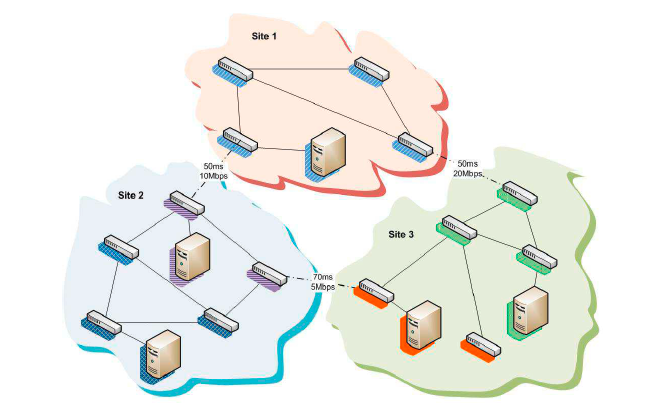
\includegraphics[scale=1]{Imagens/hiperflow.PNG} 
 
  \legend{Fonte: \citeonline{hiperflow}}
  \label{hyperflow}
\end{figure}

\par A partir dessa arquitetura todas as solicitações podem ser atendidas localmente pelos controladores, reduzindo o tráfego entre as áreas e ainda mantendo a visão global da rede. Além disso, caso algum controlador responsável por uma área falhe, outro controlador pode e irá assumir sua função, já que todos as informações necessárias estarão nos arquivos divulgados. O problema citado dessa arquitetura é justamente a necessidade de se implementar diversas instâncias do HyperFlow em cada controlador NOX, implicando em alterar o código no núcleo do controlador para interceptar comandos e serializar eventos.

\section{Onix}

A proposta de \citeonline{onix} consiste no Onix, uma aplicação para controladores distribuídos que se difere de outros trabalhos por expor uma interface mais genérica, tendo como alvo ambientes diversos como redes WAN, nuvens públicas e centros de dados corporativos.Além disso, provê meios para distribuições flexíveis permitindo que os \emph{designers} de aplicações implementem aplicações de controle sem reinventar mecanismos de distribuições e mantendo requisitos de escalabilidade e performance. De acordo com a Figura \ref{onix}, existem 4 componentes em uma rede controlada pelo Onix:

\begin{itemize}
    \item Infraestrutura física: Inclui \emph{switches} e roteadores e outras entidades físicas que permitam que Onix leia e escreva o estado que controla o comportamento do elemento, como em uma espécie de tabela de encaminhamento.
    \item Infraestrutura de conexão: Corresponde à comunicação entre o Onix e a infraestrutura física. Esse canal de controle pode ser implementando tanto na banda(tráfego de controle compartilha a mesma conexão com o tráfego de dados), como fora da banda(tráfego de controle e dados utilizam conexões separadas) e deve fornecer ainda comunicação bidirecional.
    \item Onix: Sistema distribuído que é executado em um cluster composto de um ou mais sevidores físicos, onde cada um pode executar múltiplas instâncias do Onix. O Onix é responsável por fornecer acesso lógico de controle à rede(em ações como escrever e ler o estado da rede) e disseminar o estado da rede para outras instâncias dentro do cluster.
    \item Lógica de controle: A lógica de controle da rede é implementada no topo da interface do Onix. Essa lógica determina o comportamento desejado da rede. O Onix somente fornece os meios necessários para acessar o estado apropriado da rede.
\end{itemize}


\begin{figure}[!h]
	\caption{ Arquitetura do Onix}
  \centering
  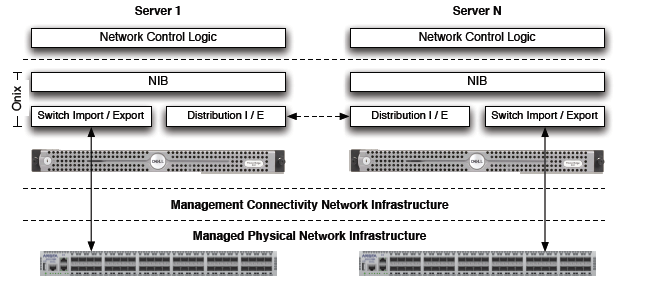
\includegraphics[scale=1]{Imagens/onix.png} 
 
  \legend{Fonte: \citeonline{onix}}
  \label{onix}
\end{figure}

O Onix utiliza um modelo de dados chamado \emph{Network Information Base} (NIB). Este modelo faz o controle do estado da rede através de uma estrutura de dados que armazena um grafo das entidades da topologia da rede. É através da replicação e distribuição desse modelo NIB que o Onix consegue prover a escalabilidade. Para que ocorra a sincronização de dados sem falha entre os processos distribuídos, o Onix utiliza a API Apache Zookeeper, possibilitando que o mesmo mantenha, por exemplo, informações de configuração, nomeação de servidores e provendo serviços para grupos específicos da rede. Apesar de sua contribuição relevante, tendo se baseado no contolador NOX e no Apache ZooKeeper, o Onix foi desenvolvido em código fechado, impossibilitando a integração e o desenvolvimento de novas aplicações.
\pagebreak
\section{DISCO - \emph{DIstributed SDN COntrol Plane} }

O trabalho de \citeonline{disco} apresenta outra possibilidade para integração de controladores DISCO. A implementação se baseia nos controladores Floodlight, cada qual com seu domínio da rede. Por sua vez estes se comunicam para manter uma visão global da rede utilizando uma interface \emph{East/West} através do \emph{Advanced Message Queuing Protocol} (AMQP)\cite{amqp}. O OpenFlow se mantém como interface \emph{SouthBound} para comunicação com a camada de dados da rede.
    O conceito utilizado pelo DISCO é que cada controlador Floodlight possui um agente configurado que permite trocar informações sobre os domínios adjacentes utilizando o AMQP. Essa API é composta de um módulo que identifica os controladores vizinhos, possibilitando a troca de mensagens. Entre os agentes descritos temos:
    
    \begin{itemize}
        \item O agente de conectividade, responsável pelo peering;
        \item O agente de monitoramento, responsável por buscar informações sobre largura de banda e latência;
        \item O agente de acessibilidade, responsável por avisar caso apareça um novo host no domínio;
        \item O agente de reserva, que utiliza o \emph{Resource reServation Protocol} (RSVP) para
        fornecer recursos fim-a-fim;
    \end{itemize}

O maior desafio relacionado ao DISCO é que este utiliza módulos exlusivos para o controlador Floodlight, tornando a aplicação dependente destes.

\section{OrchFlow}

O trabalho de \citeonline{frate} surgiu em meio aos desafios verificados em trabalhos anteriores. Ele sugere a ferramenta OrchFlow como software orquestrador para redes SDN baseadas no OpenFlow. 
  A Figura \ref{orchflow} ilustra a arquitetura do Orchflow. Ele atua como um agente integrador entre as aplicações disponíveis na rede e também entre os diversos controladores que gerenciam subdomínios sob um mesmo domínio administrativo. Na base da arquitetura temos os \emph{switches}, que formam a infraestrutura da camada de dados; e para cada conjunto de \emph{switches} temos um um subdomínio da rede que é controlado por um controlador SDN através do OpenFlow. Cada controlador está conectado ao OrchFlow através de uma interface central, que independe da linguagem de programação do controlador. Além disso, o OrchFlow possibilita a comunicação entre diferentes aplicações através da interface \emph{NorthBound}, recebendo solicitações específicas de serviços pré-determinados pelo OrchFlow. Essa integração entre aplicações e controladores só é possível porque utiliza-se uma Interface \emph{Representational State Transfer} (REST), que aplica regras estabelecidas para a aplicação solicitante e entrega para o controlador adequado, conforme seu subdomínio.O OrchFlow ainda fornece três modos de atuação: o Proativo, o Reativo e o Híbrido, que dizem respeito a forma de gerenciamento dos fluxos entre os \emph{switches}.
  
\begin{figure}[!h]
	\caption{ Arquitetura do OrchFlow}
  \centering
  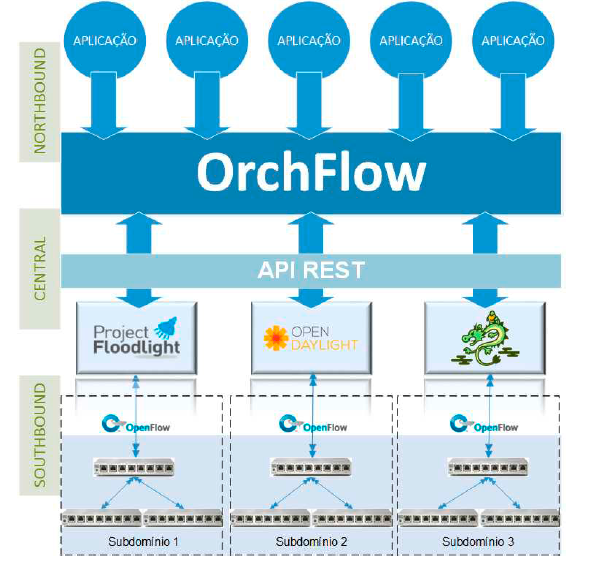
\includegraphics[scale= 0.8] {Imagens/orchflow.PNG} 
 
  \legend{Fonte: \citeonline{frate}}
  \label{orchflow}
\end{figure}

Com relação a sua implementação, a linguagem java foi escolhida para a implementação do OrchFlow. Além disso, para armazenamento dos dados, utiliza-se o banco de dados Neo4j \cite{neo}, um banco de dados orientado a grafos também baseado em Java, que oferece persistência, alto desempenho, escalabilidade e com boa documentação. 
\par A possibilidade da escalabilidade para gerenciar qualquer número de controladores implementados em qualquer linguagem, sob uma topologia hierárquica ou não e ainda com uma interface WEB torna o OrchFlow um orquestrador diferenciado, entretanto, seus testes ocorreram somente com os controladores Ryu e FLoodlight, sendo necessário mais testes para otimização de códigos com outros tipos de controladores, bem como com outros tipos de aplicações.















\chapter{Metodologia}

 Este capítulo fornece um acompanhamento da metodologia do projeto de TCC para em seguida apresentar o cronograma previsto de conclusão.
 
 \section{Pesquisa}
 
 O embasamento teórico para a escrita dos capítulos de fundamentação teórica e trabalhos relacionados se originou atráves de uma revisão de literatura em bases específicas como \emph{IEEEexplor, ACM Digital Library, Springer, Sciente Direct, Periódicos Capes e Elsevier}. A pesquisa nessas bases foi direcionada para duas áreas: Redes Definidas por Software e Segurança de Redes de Computadores. Além da leitura de artigos, livros didáticos e sites de instituições também foram utilizados como ferramentas para aprendizagem conceitual.
\par O Objetivo principal deste trabalho, já citado anteriormente, é implementar um gerenciador SDN para 2 controladores com diferentes implementações e associados a serviços diferentes. Os controladores escolhidos para esse gerenciamento possuem serviços implementados pelos trabalhos de \citeonline{bomfim2}  e \citeonline{pablo}.
\par O serviço implementado por \citeonline{pablo} se baseia no no modelo de gerência autonomômico em uma rede SDN. Ele propõe o MAdPE-k/SDN, um serviço distribuído nas camadas de infraestrutura e de aplicação da rede SDN, provendo autoproteção e autogerenciamento. O controlador utilizado foi o RYU, que possui implementação em Python. Já no trabalho de \citeonline{bomfim2}, foi desenvolvido um serviço de anonimização de endereços IP em uma rede SDN : o anonimizador BOMIP. O controlador utilizado por ele foi o RunOS, implementado em C/C++. 

\section{Ferramentas e Implementação}

\par Para a fase de experimentação e análise dos controladores, bem como para testar o gerenciador as seguintes ferramentas serão utilizadas:

\begin{itemize}
    \item Ambiente de implementação e execução na nuvem OpenStack;
    \item VMs Linux;
    \item Banco de dados (a definir);
    \item Controladores Ryu e RunOS;
    \item OpenVSwitch - Com suporte ao OpenFlow;
    \item Sistema operacional Linux (configurações a serem consultadas)
    \item Emuladores de rede Mininet e GNS3;
    \item Virtual Box;
\end{itemize}

 A linguagem de programação para o desenvolvimento do módulo será um dos pontos a serem definidor após a análise da arquitetura dos controladores a serem gerenciados.


 \section{Cronograma}
 
 
  
 \begin{table}[h]
 \begin{center}
 \caption{Plano para continuidade do TCC2}
\begin{tabular}{p{6cm} | c|c|c|c|c|c}
\hline 
\textbf{Atividade} & Abril & Maio & Junho & Julho & Agosto & Setembro \\ \hline 
Análise do controlador Ryu com o serviço com autonomicidade & X &  &  &  & & \\ \hline
 Análise do controlador RunOS com o serviço de anonimização & & X & & & &\\ \hline
Implementação do módulo gerenciador & & & X & X & X &\\ \hline
 Testes, obtenção de resultados e apresentação & & & & X & X & X\\ \hline

\end{tabular}
\end{center}
\label{cronograma}
\end{table}




\bibliography{Bibliografia}

% ----------------------------------------------------------
% ELEMENTOS PÓS-TEXTUAIS
% ----------------------------------------------------------
\postextual

\renewcommand{\chapnumfont}{\chaptitlefont}
\renewcommand{\afterchapternum}{}
%\begin{apendicesenv}

% Imprime uma página indicando o início dos apêndices
\partapendices

% ----------------------------------------------------------
\chapter{}
% ----------------------------------------------------------

\lipsum[50]

% ----------------------------------------------------------
\chapter{}
% ----------------------------------------------------------
\lipsum[55-57]

\end{apendicesenv}

%\begin{anexosenv}


% Imprime uma página indicando o início dos anexos
\partanexos

% ---
\chapter{}
% ---
\lipsum[30]

% ---
\chapter{}
% ---

\lipsum[31]

% ---
\chapter{}
% ---

\lipsum[32]


\end{anexosenv}


\end{document}